\documentclass[a4paper,12pt]{article}
\usepackage[utf8]{inputenc}
\usepackage{graphicx}

%\usepackage{epsfig}

\begin{document}

\author{Istvan Elek}
\title{DEM Center Users' Guide}
\date{2022}

%\frontmatter
\maketitle
\newpage
\tableofcontents
\newpage
%\mainmatter


\section{Preface}

DEM centre is a program package written in C\#, which is the heart of digital evolution. You can create any size of labyrinths with any DEM workers and wumpuses, traps and gold. The system  helps you to understand what happened to  evolutional workers in this peculiar world. The system saves all events and workers into a Postgres database, so PostgreSQL 9.6 or later version has to be installed previously. PgAdmin is optional, but very useful tool, so it is also suggested to install. Use the Master to start thousands of DEM workers to discover the world. Start Analyser in order to understand the events.



\section{Installation}

\begin{enumerate}
	\item Download the ziped (dc.zip) package from this site (Download menu)
	\item Copy it to the desired directory and unzip
	\item Download Postgres 9.6 or later version and install it
	\item Download and install pgAdmin 4.x (optional)
	\item Create a postgres user with name: wumpus with password: wumpus with admin rights (use postgres command line or pgAdmin). If you want to use your own parameters, open \textit{config.cfg} file, from the program directory and put your data into it (username: wumpus,	password: wumpus, 	host: localhost). You may also need to change the content of \textit{configAdmin.cfg} file (username postgres, password root, database postgres, host localhost) if your data are different from them.
	\item Start DC.exe
	\item Let's start the simulation.
\end{enumerate}



\section{DC}

DC.exe is a frame program, which organize your work. You can make the followings (Figure \ref{fig:dcstart}):

\begin{figure}
	\centering
	\includegraphics[width=2cm]{dcstart.png}
	\caption{DC Centre form: Demo,  Master, Analyser modules can be launched from here.}
	\label{fig:dcstart}
\end{figure}



\begin{itemize}
	\item You can start DCDemo.exe, which demonstrates graphically the movements of DEM entities (workers) in small labyrinth. There is no database connection and knowledge base creation in this case.
	\item If you are going to make simulations, start DCMaster.exe.
	\item If you already have simulation results, you can use DCAnalyser.exe to analyse databases, to understand what have happened to evolutional entities, and what the fate of DEM workers is.
\end{itemize}

The easiest way to start click to DC.exe, and start further modules from here.



\section{DCDemo}

DCDemo.exe  demonstrates graphically the movements of DEM entities (workers) in small labyrinth (Figure \ref{fig:demo}). There is no database connection and knowledge base creation in this case. Here you can create workers, any sized labyrinth with many wumpuses, traps and gold bars. Do not create to much (suggested only one), because picture may become confusing.
If worker has died the live flag emphasized with black colour. If the worker found gold, the live flag became green, the 'gotcha' flag turns \textit{true} emphasized with green colour.

\begin{figure}
\centering
	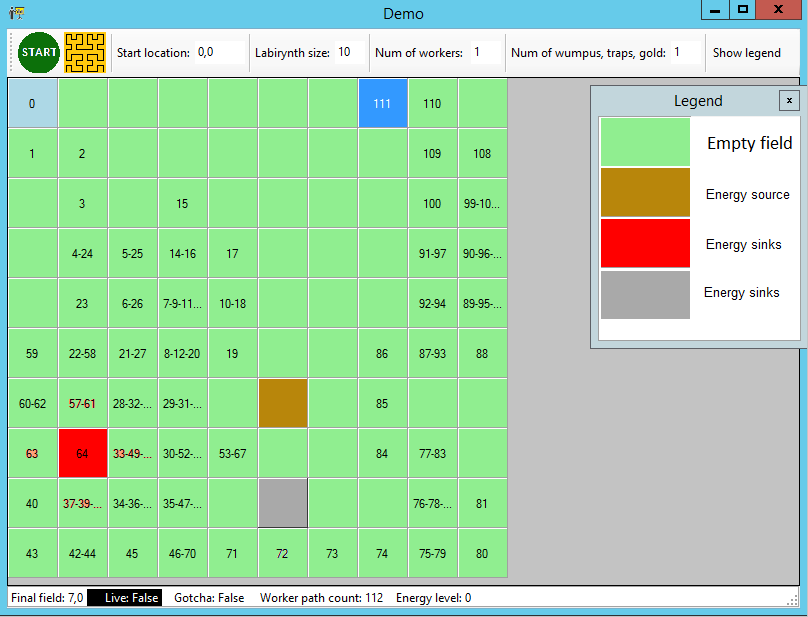
\includegraphics[width=14cm]{demo.png}
	\caption{DCDemo: Labyrinth with legend and movements can be seen. Numbers symbolize the step number when the certain field was entered.}
	\label{fig:demo}
\end{figure}




\section{DCMaster}

\begin{figure}
	\begin{center}
		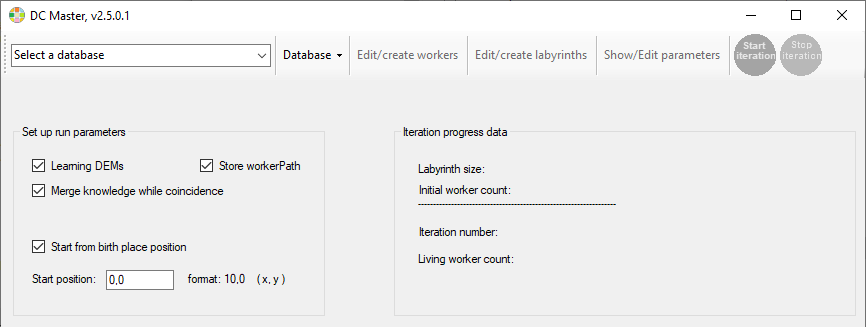
\includegraphics[width=15cm]{master1.png}
		\caption{The DCmaster starter screen: This is where you can open an existing database (invasion) or create any labyrinths, DEM workers, and you can set up simulation parameters. }
		\label{fig:master1}
	\end{center}
\end{figure}

If you are going to make simulations, start DCMaster.exe (Figure \ref{fig:master1}). First, you need to create a new database (simulation) in the \textit{Database} menu (Figure \ref{fig:menu_database}). Also in it you can edit/display config file (Figure \ref{fig:config}), which contains connection parameters to Postgres and existing wumpus databases. 

After creation you should select this new database. Click to 'Select a database' combo box to select the desired database.
If you created a new database (new simulation), or you selected an existing one,  you can create DEM workers by clicking \textit{Edit/Create workers} menu (Figure \ref{fig:menu_create_workers}). 
You can also create any size of labyrinth by clicking \textit{Edit/Create labyrinths} menu (Figure \ref{fig:mnu_createlabs}), or edit existing one. You can set the size of  labyrinths, and the number of wumpuses, traps and gold bars in it. 



%You can chose operation modes too, such as use machine learning, or not use. You can set up starting position by hand or by random method. After you clicked to \textit{StartInvasion} button you can see summary data after every closed session in 'Workflow progress data' section.



\begin{figure}
	\begin{center}
		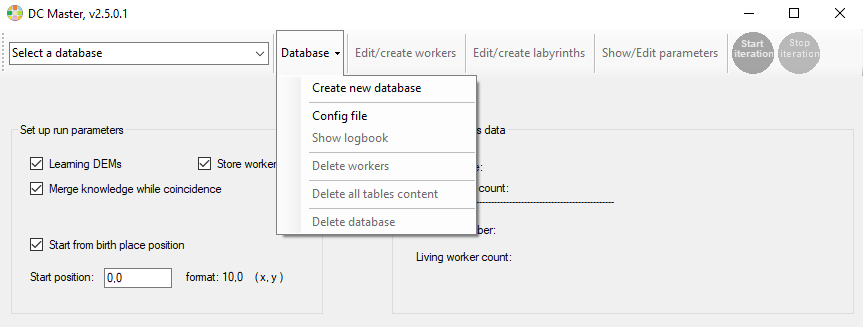
\includegraphics[width=11cm]{menu_database.png}
		\caption{Database menu, where you can create new database, or edit config file}
		\label{fig:menu_database}
	\end{center}
\end{figure}

\begin{figure}
	\begin{center}
		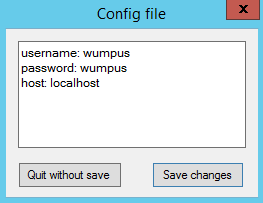
\includegraphics[width=6cm]{config.png}
		\caption{Database/Config file menu, where you can edit/view the config file content}
		\label{fig:config}
	\end{center}
\end{figure}

\begin{figure}
	\begin{center}
		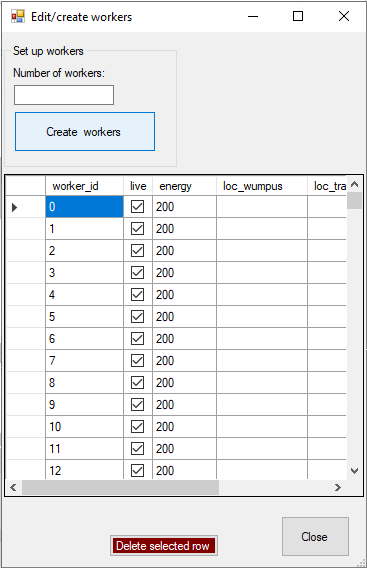
\includegraphics[width=8cm]{menu_create_workers.png}
		\caption{Edit/Create worker menu: here you can create or delete the selected workers. The number of workers has to be set up before clicking to 'Create workers' button., }
		\label{fig:menu_create_workers}
	\end{center}
\end{figure}

\begin{figure}
	\begin{center}
		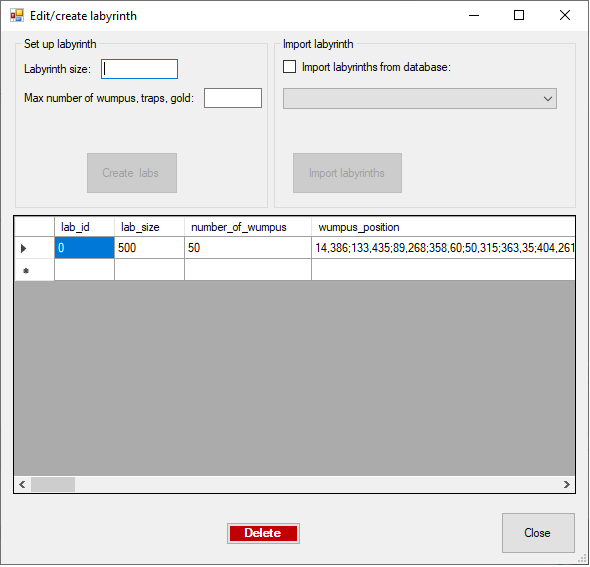
\includegraphics[width=12cm]{mnu_createlabs.png}
		\caption{Edit/Create labyrinth menu: here you can create any size of labyrinths with any number of wumpuses, traps and gold bars.}
		\label{fig:mnu_createlabs}
	\end{center}
\end{figure}

 
You can set up parameters (Figure \ref{fig:mnu_showparameters}) of the world: initial worker energy, movement costs, wumpus, trap, gold energy content, replication energy level, replication rate (default is 2), etc. 

\begin{figure}
	\begin{center}
		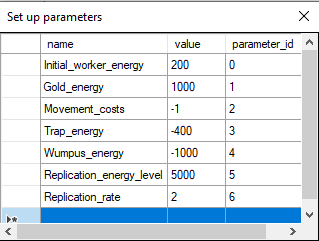
\includegraphics[width=7cm]{mnu_showparameter.png}
		\caption{Set up parameters menu is for adjusting the circumstances in the artificial world (labyrinths). You can edit world parameters if you change values. The changed value is stored if you select the next record.}
		\label{fig:mnu_showparameters}
	\end{center}
\end{figure}


In the \textit{Database} menu there are three further sub menus. The first is \textit{Delete workers}, which delete all existing workers from the invasion database and worker related table such as worker\_path and knowledge. It is useful if you wish to start a new invasion with new workers, but in old labyrinths. To click to \textit{Delete all tables content} menu item deletes every table's content from the selected (actual) database such as workers, labyrinths, logbook, worker\_path. %Finally, you can display logbook content by clicking the \textit{Show logbook} menu.

If every necessary parameter has been set up, and labs and workers have been created you can start the simulation by clicking to  \textit{Start iteration} button. You can observe  events in the main form, where you can see the labyrinth size, initial workers' count, current iteration number and living worker count. The better way of observation is to start DCAnalyser.exe which has many functions to display and analyse data.

If you want to cancel the simulation process, click to \textit{Stop iteration} button. Every simulation has a report file where the main metadata are store after the process interruption (either stopped by the user or the living worker number became zero).

\section{DCAnalyser}


If you already have simulation results, or you have just started the simulation process by clicking \textit{Start iteration} button, you can use DCAnalyser.exe to analyse databases (invasions data), to observe events, to understand what happened to evolutional entities, and what the fate of DEM workers are. There are built-in queries, charts and picture to help your understanding. You can create your own selections too (\textit{Sql} menu), and you can display results (\textit{Diagrams} menu). In \textit{Selection} menu you can see discovered fields of a labyrinth. Figure \ref{fig:analyser} demonstrates the complexity of DCAnalyser. You can see a labyrinth not only in tabular form, but in graphics too if you click to a labyrinth with right mouse button.


\begin{figure}
	\begin{center}
		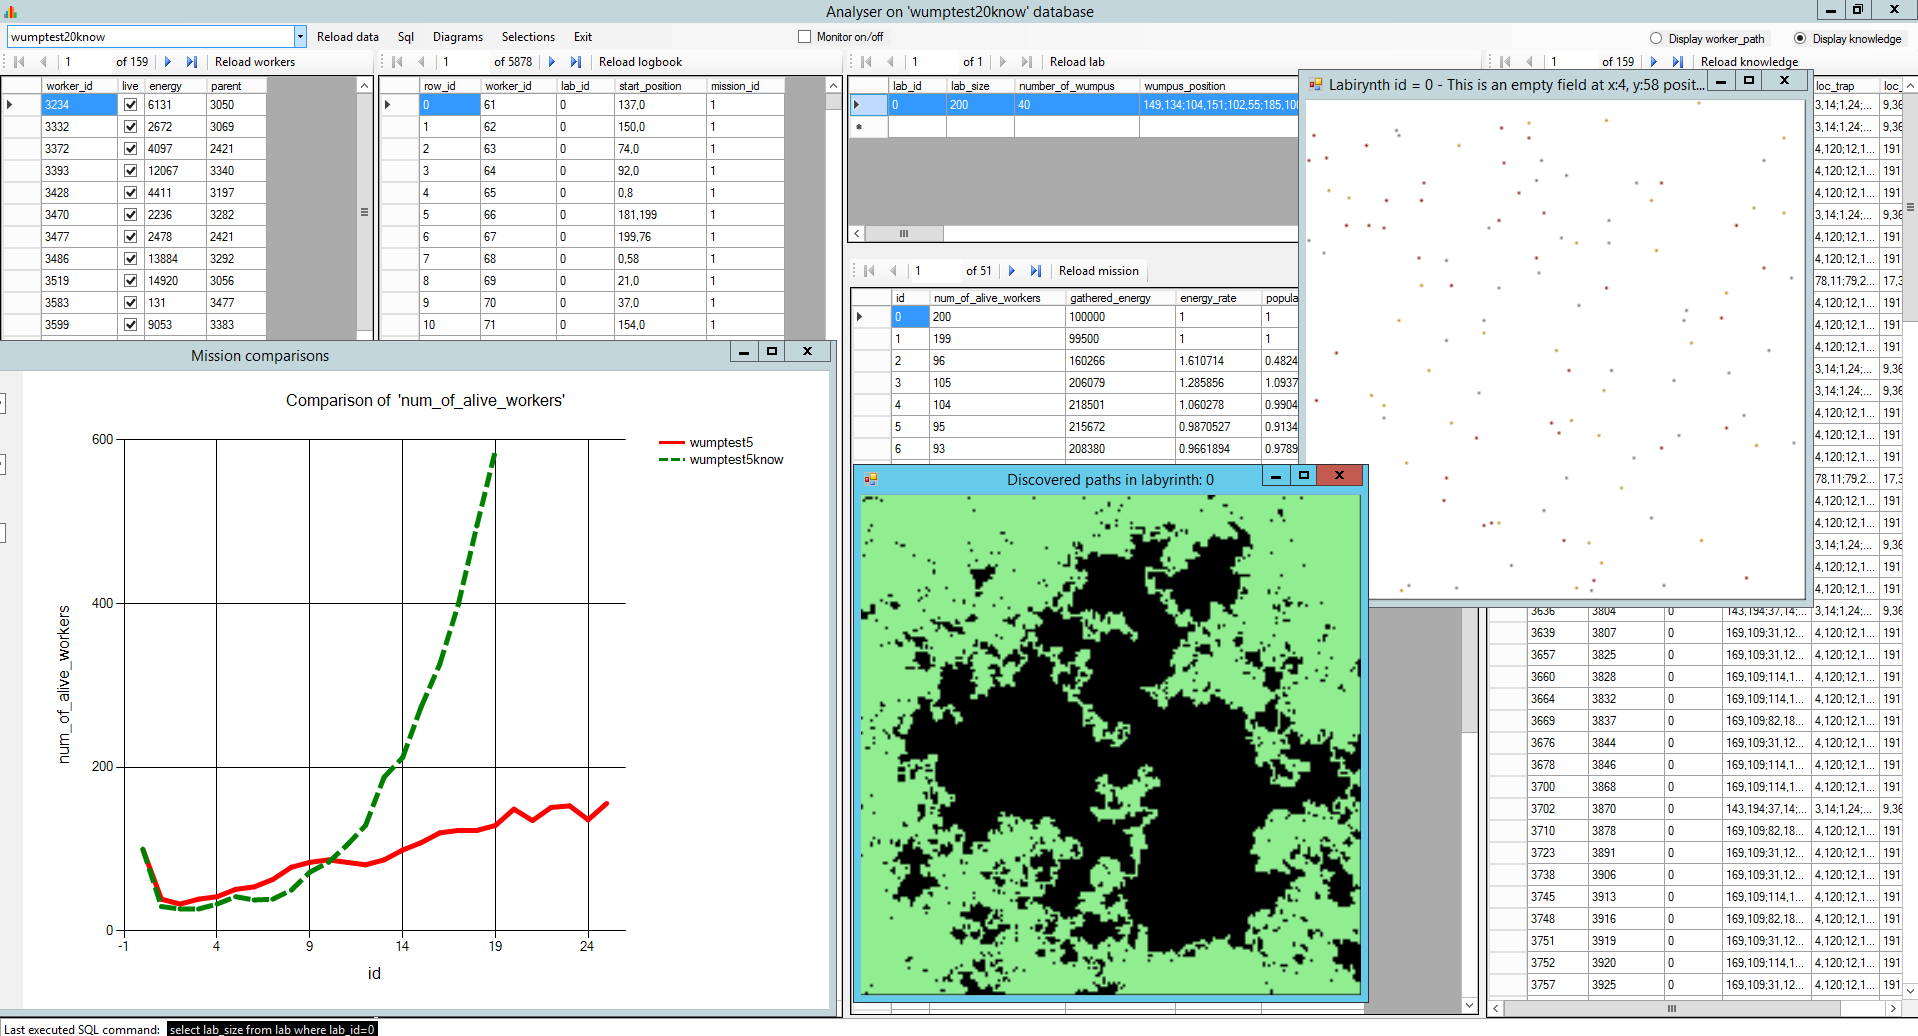
\includegraphics[width=15cm]{analyser1.png}
		\caption{DCAnalyser: This module has wide range functions of data analysis. You can see data in tabular form, and graphics too, such as charts or images}
		\label{fig:analyser}
	\end{center}
\end{figure}


After DCAnalyser.exe start you need to analyse the database. Select a database (simulation) to analyse events and data (Figure \ref{fig:dcaselect}). When a database has been selected its content were loaded to different tables (workers, logbook, labyrinths, worker-Path). 
%If you checked 'Display knowledge' (Figure \ref{fig:check_displayknowledge}), you will see workers' knowledge in the datagridview. If you checked 'Display worker path' you will see the the worker path of all workers.


\begin{figure}
	\begin{center}
		\includegraphics[width=9cm]{dcaselect.png}
		\caption{Click to 'Select a database' combo to select a database which contains every data of the selected simulation}
		\label{fig:dcaselect}
	\end{center}
\end{figure}

After selection of a database the main menu becomes enable. \textit{Data menu} item allows you to reload database names or tables' content if a new simulation database was created in \textbf{DCMaster}, and you are going to observe it. If currently a completed simulation database is open you can see the simulation report.


\begin{figure}
	\begin{center}
		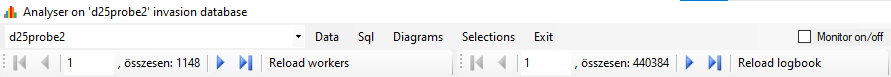
\includegraphics[width=14cm]{dcamainmenu}
		\caption{This the main menu of DCAnalyser. }
		\label{fig:dca_main}
	\end{center}
\end{figure}


\begin{figure}
	\begin{center}
		\includegraphics[width=6cm]{mnureloadata}
		\caption{This the main Data menu. Here you can reload simulation data, and see the simulation report. }
		\label{fig:dca_main}
	\end{center}
\end{figure}


\begin{figure}
	\begin{center}
		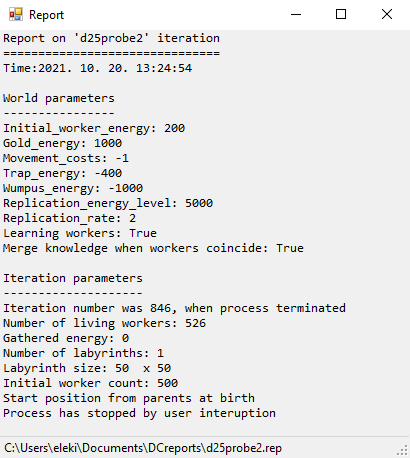
\includegraphics[width=8cm]{simreport}
		\caption{A simulation report }
		\label{fig:simreport}
	\end{center}
\end{figure}

%The selected database content should be reloaded (Figure \ref{fig:mnuReloadata}), if the content of selected database is changing (for example a simulation is running just now). 

If you check the monitor option  in main menu bar you can observe the number of alive workers in real time, during the simulation.




%\begin{figure}
%	\begin{center}
%		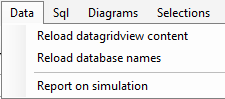
\includegraphics[width=5cm]{mnuReloadata.png}
%		\caption{Reload menu: You can reload the selected database content. You can also reload database names. It is needed if you started a new simulation with DCMaster.exe, and a new simulation database has been created.}
%		\label{fig:mnuReloadata}
%	\end{center}
%\end{figure}

You can make any selections with \textit{Sql} menu (Figure \ref{fig:mnusql}). if you know Sql you can create your own Sql query, and you can see it in tabular form. If you choose \textit{Display charts from any Select} sub menu you can see the result in chart form.

\begin{figure}
	\begin{center}
		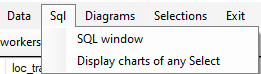
\includegraphics[width=7cm]{mnusql.png}
		\caption{With Sql menu you can create arbitrary Sql selections. You can display results in tabular or graphic form}
		\label{fig:mnusql}
	\end{center}
	\end{figure}


In \textit{Diagram} menu (Figure \ref{fig:mnudiagrams}) you can see simulation data on charts: population (number of alive workers), population rate, gathered energy, energy rate, and fitness of groups. You can also compare any data from any simulation. If you click to the special icon (white arrows) an sql command field displays, where you can see actual Sql statement.

You can not only display charts on the certain database (simulation), but compare data of different simulations (Figure \ref{fig:comparison}). If you choose \textit{Compare simulations} menu you can choose desired simulation database name and data type to display.

\begin{figure}
	\begin{center}
		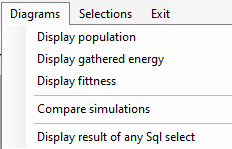
\includegraphics[width=6cm]{mnudiagrams.png}
		\caption{You can draw charts if you choose any sub menus from \textit{Diagram} menu. }
		\label{fig:mnudiagrams}
	\end{center}
\end{figure}

\begin{figure}
	\begin{center}
		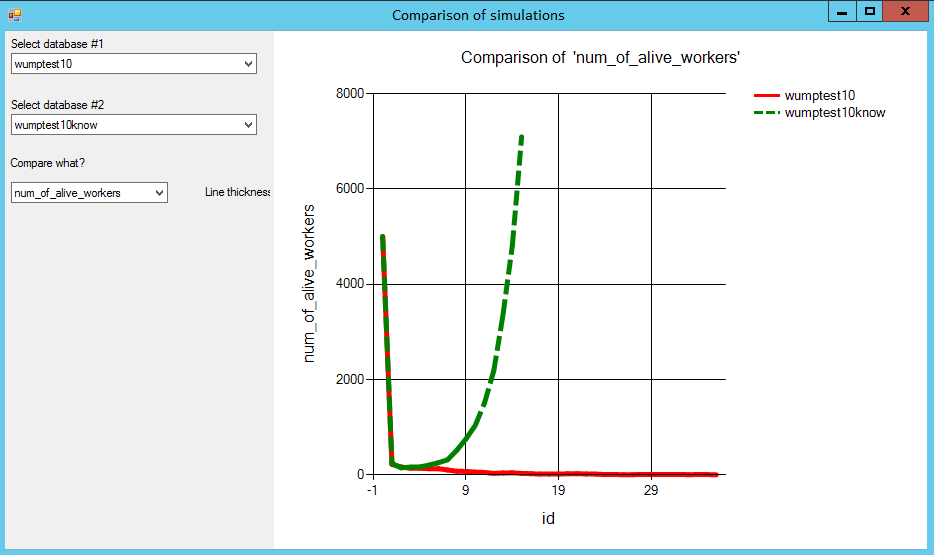
\includegraphics[width=15cm]{comparison.png}
		\caption{Comparison of two simulation databases.}
		\label{fig:comparison}
	\end{center}
\end{figure}
		
\begin{figure}
	\begin{center}
		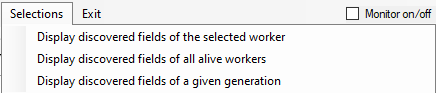
\includegraphics[width=10cm]{mnuselections.png}
		\caption{Selection menu: here you can select worker specific knowledge and display discovered fields.}
		\label{fig:mnuselections}
	\end{center}
\end{figure}

Choose \textit{Selections} menu (Figure \ref{fig:mnuselections}) if you wish to see workers' knowledge for selected labyrinth or for all labyrinth. If the workers knowledge is interesting, first you should select a certain worker by clicking to a record in'workers' table. If you did not select labyrinth the selected knowledge is valid for all labyrinths.

In \textit{Selections} menu you can display the discovered fields of a selected labyrinth (Figure \ref{fig:discoverlab1}). You can see individual or collective knowledge as an image. The union of individual results is the collective knowledge.


\begin{figure}
	\begin{center}
		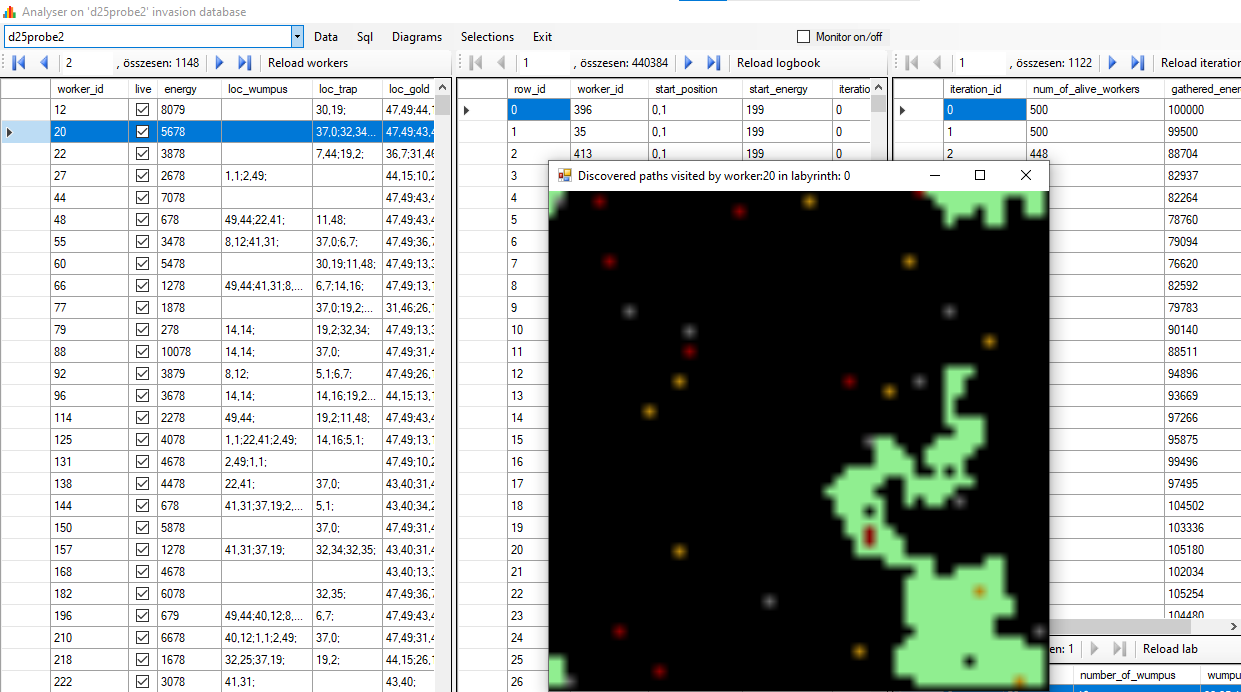
\includegraphics[width=13cm]{discoverlab1.png}
		\caption{Discovered fields (green pixels) by a selected worker in a certain labyrinth. Gold pixels are gold bars, red pixels are traps and grey pixels are wumpuses}
		\label{fig:discoverlab1}
	\end{center}
\end{figure}

You can see a labyrinth graphically if you make a mouse click with right mouse button to a record in lab table data grid view. I  this was you will see the distribution of objects in the selected labyrinth (Figure \ref{fig:labrightclick}).

\begin{figure}
	\begin{center}
		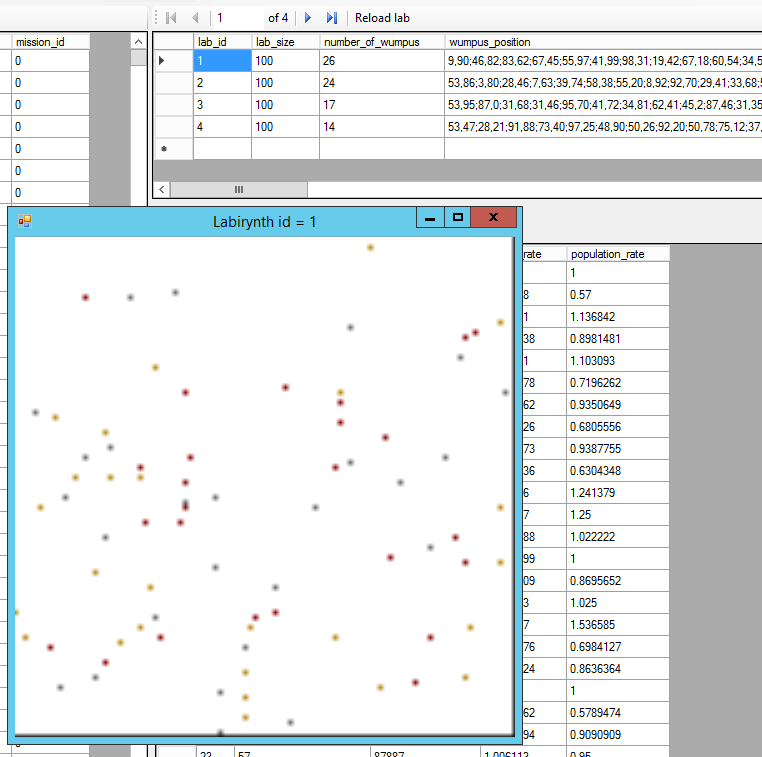
\includegraphics[width=15cm]{labrightclick.png}
		\caption{A certain labyrinth with many wumpuses (dark grey points), traps (red points) and gold bars (goldenrod points). Select a labyrinth by clicking with right mouse button on lab datagrid if you wish to see the labyrinth graphically.}
		\label{fig:labrightclick}
	\end{center}
\end{figure}

\end{document}